\section{Hardware}
\subsection{Raspberry PI}
The Raspberry PI is a small computer in the form of a system on a chip. It has an ARM11v6 CPU running at 700 MHz.
\begin{figure}
    \centering
    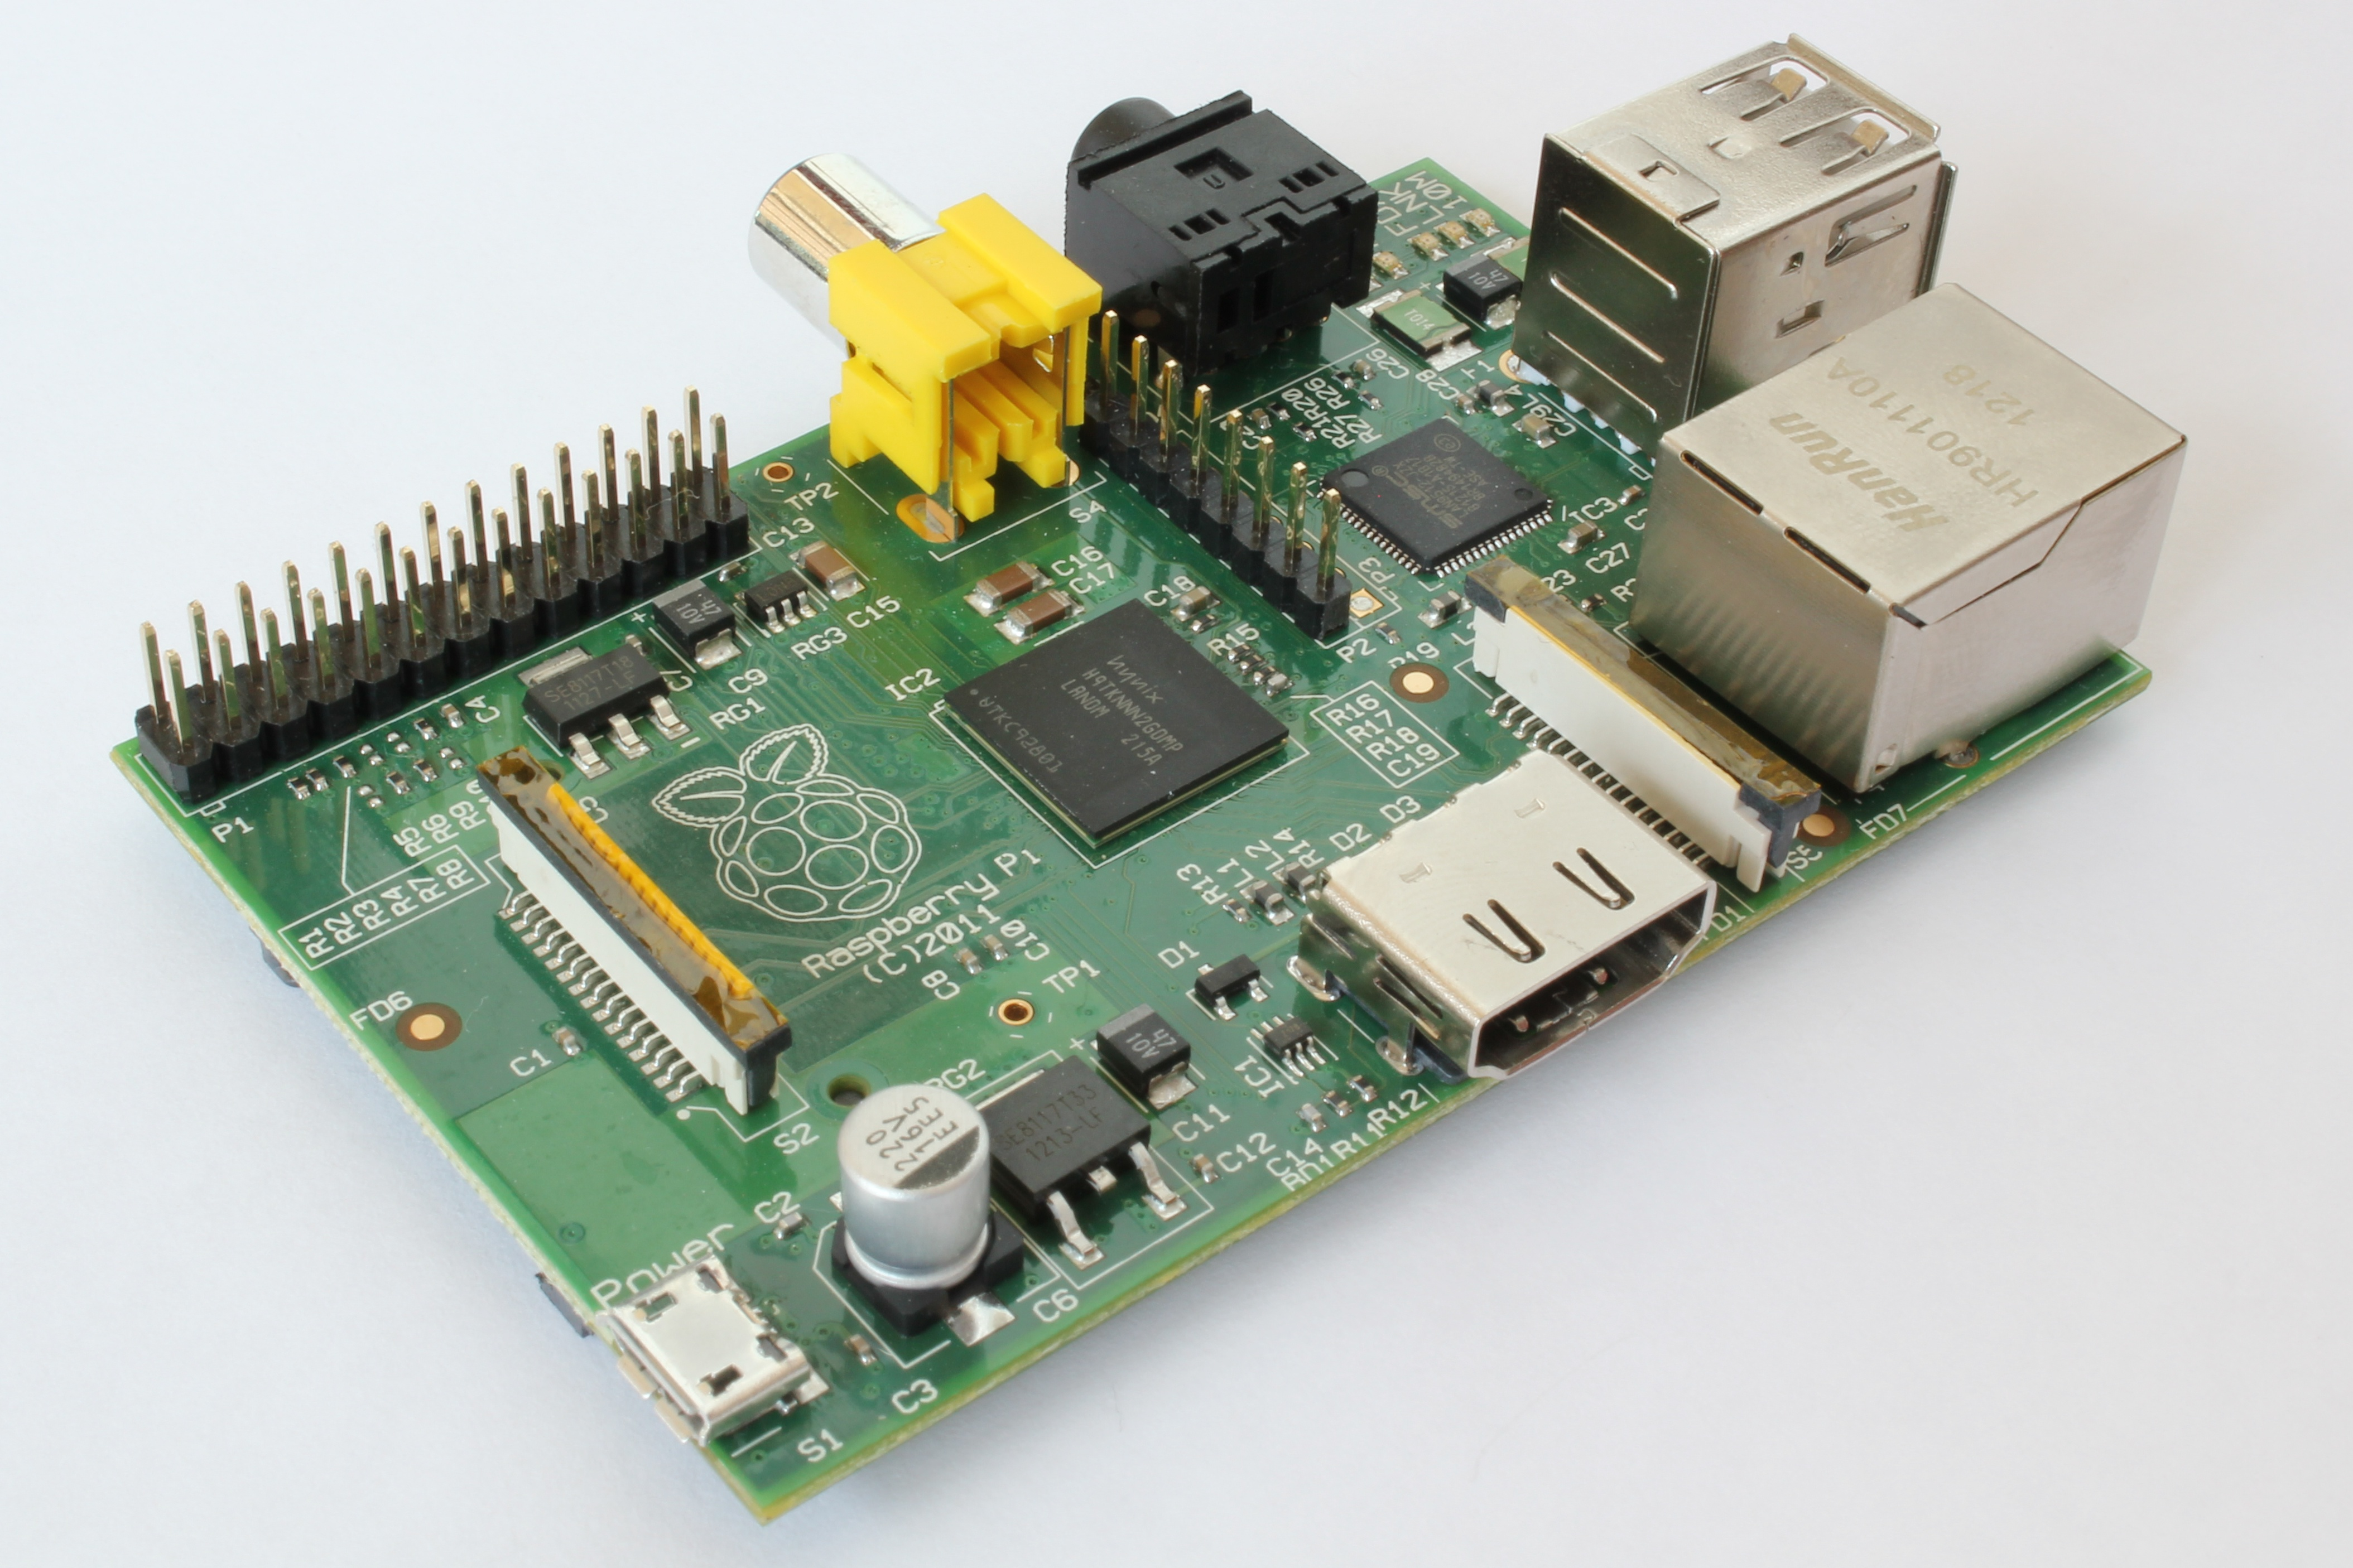
\includegraphics[width=0.5\textwidth]{hardware/RaspberryPi}
    \caption{A Raspberry PI}
    \label{fig:raspberrypi_hw}
\end{figure}

\subsection{Alternative hardware}
\subsubsection{BeagleBone Black}
The BeagleBone Black is another open source low power mini pc on a single board. It is made by Texas Instruments and sold under the Creative Commons license.
The board is made from an AM3359 SoC from Texas Instruments, sporting an ARMv7 Cortex-A8 running at 1 GHz with 512MB of DDR3 RAM. This board has a slightly weaker GPU than the PI, which is of interest as we will not be using it anyway, and could help giving more power to the CPU.
We did not know about the release of this board when we did the planning for this project, but with it's very similar pricing (\$45 as of this writing) and significantly more powerful CPU, it would make for an interesting comparison and alternative.
\subsubsection{MK802}

\subsection{Cluster}
\subsection{Power}
